% Intended LaTeX compiler: pdflatex
\documentclass[a5paper]{memoir}
\makeatletter

\usepackage{vocabulary}

\def\maketitle{}

\usepackage{eso-pic}

\newcommand*{\casesLegendHeaderBG}{%
  \AddToShipoutPictureBG{%
    \put(\LenToUnit{\paperwidth-25mm-\spinemargin},\LenToUnit{\paperheight-84mm}){%
      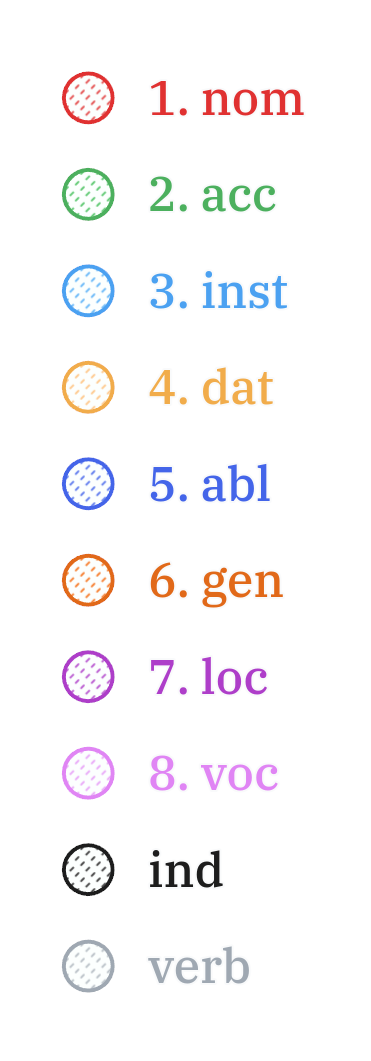
\includegraphics[width=25mm]{./images/cases-legend-white-large.png}%
    }%
  }%
}

\newcommand*{\casesLegendHeaderBGHere}{%
  \AddToShipoutPictureBG*{%
    \put(\LenToUnit{\paperwidth-25mm-\spinemargin},\LenToUnit{\paperheight-84mm}){%
      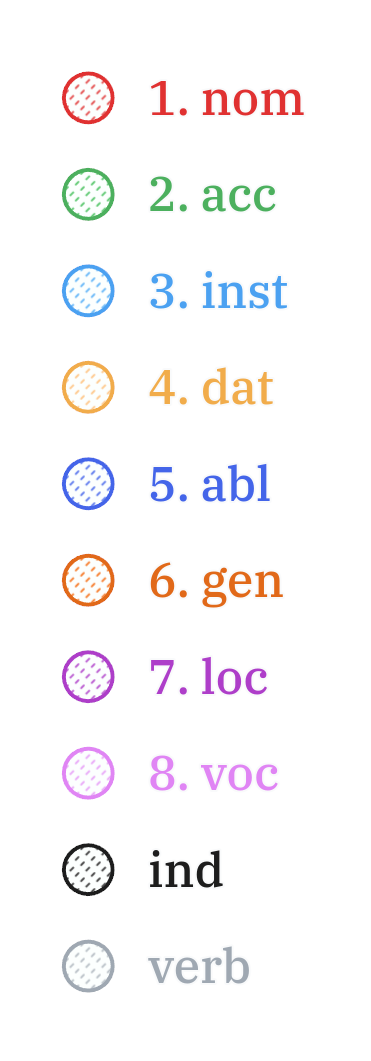
\includegraphics[width=25mm]{./images/cases-legend-white-large.png}%
    }%
  }%
}


\makeatother

\setcounter{secnumdepth}{2}
\date{\today}
\title{Vocabulary: Lesson 1}
\hypersetup{
 pdfauthor={The Bhikkhu Saṅgha},
 pdftitle={Vocabulary: Lesson 1},
 pdfkeywords={},
 pdfsubject={},
 pdfcreator={Emacs 30.0.50 (Org mode 9.6.6)}, 
 pdflang={English}}
\begin{document}


\chapter{Vocabulary}
\label{sec:org377b529}

\begin{longtable}{L{0.48\linewidth} L{0.48\linewidth}}
a cook & sūda (m.)\\[0pt]
rice & bhatta (m.)\\[0pt]
he cooks & pacati\\[0pt]
The chef cooks the rice. & Sūdo bhattaṁ pacati.\\[0pt]
boy & dāraka (m.)\\[0pt]
food (lit. an enjoyable) & bhojanīya (m.)\\[0pt]
eats; enjoys & bhuñjati\\[0pt]
The boys eat the food. & Dārakā bhojanīyaṁ bhuñjanti.\\[0pt]
bird & sakuṇa (m.)\\[0pt]
sky & ākāsa (m.)\\[0pt]
flies up; files off; flies away & uḍḍayati\\[0pt]
Birds fly in the sky. & Sakuṇā ākāse uḍḍayanti.\\[0pt]
horse & assa (m.)\\[0pt]
white & seta (adj.)\\[0pt]
here & idha (ind.)\\[0pt]
there & tattha / tatra (ind.)\\[0pt]
now & idāni (ind.)\\[0pt]
before, previously & pubbe (ind.)\\[0pt]
after & pacchā (ind.)\\[0pt]
heavenly being; a god & deva (m.)\\[0pt]
form & rūpa (nt.)\\[0pt]
feeling & vedanā (f.)\\[0pt]
I (pron.) & ahaṁ\\[0pt]
we & mayaṁ\\[0pt]
you (sg.) & tvaṁ\\[0pt]
you (pl.) & tumhe\\[0pt]
he & so, sa (m.)\\[0pt]
they (m.) & te (m.)\\[0pt]
it & taṁ, tad (nt.)\\[0pt]
they (nt.) & tāni (nt.)\\[0pt]
she (f.) & sā (f.)\\[0pt]
they (f.) & tā, tāyo (f.)\\[0pt]
he who (m.nom.) & yo (m.)\\[0pt]
to me & maṁ\\[0pt]
speaks & bhāsati\\[0pt]
She speaks to him/them. & Sā taṃ bhāsati.\\[0pt]
sick; ill; unwell & gilāna (adj.)\\[0pt]
attends & upaṭṭhāti\\[0pt]
he who attends to the ill & yo gilānaṃ upaṭṭhāti\\[0pt]
he attends to me & so maṃ upaṭṭhāti\\[0pt]
hatred; hostility & vera (nt.)\\[0pt]
friendliness; lit. non-hatred & avera (nt.)\\[0pt]
knows & jānati\\[0pt]
I don't know. & Na jānāmi.\\[0pt]
does & karoti\\[0pt]
you did (irregular) & akāsi\\[0pt]
Don't you do! & Mā akāsi!\\[0pt]
goes & gacchati\\[0pt]
comes & āgacchati\\[0pt]
Do you go? & Api nu / Kiṁ gacchasi?\\[0pt]
What is your name? & Kiṁ nāmo si?\\[0pt]
man & nara (m.)\\[0pt]
runs & dhāvati\\[0pt]
walks & carati\\[0pt]
chews & khādati\\[0pt]
sees & passati\\[0pt]
recites & uddisati\\[0pt]
gives & deti\\[0pt]
informs & āroceti\\[0pt]
confesses & āvikaroti\\[0pt]
I am (√as) & asmi\\[0pt]
we are (√as) & asma\\[0pt]
you are (√as) & asi\\[0pt]
you all are (√as) & attha\\[0pt]
he is (√as) & atthi\\[0pt]
they are (√as) & santi\\[0pt]
this; he; it & esa (pron.)\\[0pt]
not this I am & n'eso'ham'asmi [na + eso + ahaṁ + asmi]\\[0pt]
I am (√hū) & homi\\[0pt]
we are (√hū) & homa\\[0pt]
you are (√hū) & hosi\\[0pt]
you all are (√hū) & hotha\\[0pt]
he is (√hū) & hoti\\[0pt]
they are (√hū) & honti\\[0pt]
sits & nisīdati\\[0pt]
stands & tiṭṭhati\\[0pt]
gets up; gets out; arouses oneself; lit. stands up & uṭṭhahati; uṭṭhāti\\[0pt]
The man sits. & Naro nisīdati.\\[0pt]
The boy stands. & Dārako tiṭṭhati.\\[0pt]
The woman stands up. & Mātugāmo uṭṭhahati.\\[0pt]
lion & sīha (m.)\\[0pt]
The lions are not running. & Sīhā na dhāvanti.\\[0pt]
(is) born & jāyati\\[0pt]
the born & jāta (pp. of jāyati)\\[0pt]
dies & mīyati\\[0pt]
The born die. & Jātā mīyanti.\\[0pt]
bowl; cup & mallaka (m.)\\[0pt]
breaks; splits; shatters & bhindati\\[0pt]
The cup breaks. & Mallako bhindati.\\[0pt]
old age; growing old; decay & jara (m.) [√jar + a]\\[0pt]
disintegration; decay; old age; lit. going away & vaya (m.) [vi + √i + *a]\\[0pt]
falls & nipatati\\[0pt]
Old age falls. & Vayo nipatati.\\[0pt]
requisite; everyday item & parikkhāra (m.)\\[0pt]
practices; engages (in) & paṭisevati\\[0pt]
I use the requisite. & Parikkhāraṁ paṭisevāmi.\\[0pt]
seed; germ & bīja (nt.)\\[0pt]
The birds eat the seeds. & Sakuṇā bījāni bhuñjanti.\\[0pt]
dog & sunakha (m.)\\[0pt]
cat & biḷāra (m.)\\[0pt]
The lion doesn't see the dogs. & Sīho sunakhe na passati.\\[0pt]
moon & canda (m.)\\[0pt]
barks & bhussati\\[0pt]
The dogs are barking at the moon. & Sunakhā candaṁ bhussanti.\\[0pt]
disciple; pupil; follower & sāvaka (m.)\\[0pt]
The disciple eats the lion. & Sāvako sīhaṁ khādati.\\[0pt]
The lion eats the disciple. & Sīho sāvakaṁ khādati.\\[0pt]
fills up & paripūreti\\[0pt]
ocean & sāgara (m.)\\[0pt]
They fill up the ocean. & Paripūrenti sāgaraṁ.\\[0pt]
root (of a tree); base; foot & mūla (nt.)\\[0pt]
The māluva-seed falls at the base of sal trees. & Māluvābījaṁ sālamūle nipatati.\\[0pt]
walking tour; walking journey & cārikā (f.)\\[0pt]
wanders on tour; walks about & cārikaṁ carati (idiom.)\\[0pt]
The Buddha was wandering in the land of the Kosalans\ldots{} & Bhagavā kosalesu cārikaṁ carati\ldots{}\\[0pt]
elder; senior monk & thera (m.)\\[0pt]
The elder is going on a walk. & Thero cārikaṁ carati.\\[0pt]
layman; male lay follower & upāsaka (m.)\\[0pt]
laywoman; female lay follower & upāsikā (f.)\\[0pt]
village; hamlet & gāma (m.)\\[0pt]
The layman doesn't go to the village. & Upāsako gāmaṁ na gacchati.\\[0pt]
approaches; goes to; visits & upasaṅkamati\\[0pt]
We go up to the layman. & Upāsakaṁ upasaṅkamāma.\\[0pt]
granary; treasury; storehouse & koṭṭhāgāra (nt.)\\[0pt]
The men run to the barn. & Narā koṭṭhāgāraṁ dhāvanti.\\[0pt]
tree & rukkha (m.)\\[0pt]
The birds fly to the sal trees. & Sakuṇā sālarukkhe uḍḍayanti.\\[0pt]
dwelling; building; house & agāra (nt.)\\[0pt]
enters; goes into & pavisati\\[0pt]
We enter the hut. & Agāraṁ pavisāma.\\[0pt]
community; monastic order & Saṅgha (m.)\\[0pt]
observance day & uposatha (m.)\\[0pt]
The Sangha performs the uposatha. & Saṅgho uposathaṁ karoti.\\[0pt]
offence; transgression & āpatti (f.)\\[0pt]
He confesses the offense. & Āpattiṁ āvikaroti.\\[0pt]
empty of; devoid of; without & suñña (adj.)\\[0pt]
empty dwelling & suññāgāra (nt.)\\[0pt]
I enter the empty hut. & Suññāgāraṁ pavisāmi.\\[0pt]
We go to the roots of trees. & Rukkhamūle gacchāma.\\[0pt]
The 4 foundations of mindfulness fulfil the 7 factors of enlightenment. & Cattāro satipaṭṭhānā satta bojjhaṅge paripūrenti.\\[0pt]
The dogs are barking at the cats. & Sunakhā biḷāre bhussanti.\\[0pt]
\end{longtable}

\chapter{Extra Challenge}
\label{sec:org0063212}

\begin{longtable}{L{0.48\linewidth} L{0.48\linewidth} H}
(1) here; now; in this world; (2) in this case & idha (ind.) & \\[0pt]
master; gentleman; sir & ayya (m.) & \\[0pt]
May he come here. (imperative) & Idha āgacchatu. & s\\[0pt]
May the master come here. (imperative) & Ayyo idha āgacchatu. & \\[0pt]
Venerable, may the master come and sit here. & Bhante, ayyo āgacchatu, idha nisīdatu. & \\[0pt]
I hope; I trust & kacci (ind.) & \\[0pt]
I hope you are\ldots{} & kacci'si [kacci + asi] & \\[0pt]
bearable; tolearable & khamanīya (adj.) & \\[0pt]
able to keep going; sustainable & yāpanīya (adj.) & \\[0pt]
I hope you're keeping well Ven., I hope you're getting by? & Kacci, bhante, khamanīyaṁ kacci yāpanīyaṁ? & \\[0pt]
few; not much & appa (adj.) & \\[0pt]
fatigue; tiredness & kilamatha (m.) & \\[0pt]
worn out; tired & kilanta (adj) & \\[0pt]
little fatigue; little tiredness & appakilamatha (m.) & \\[0pt]
long road; journey & addhāna (nt.) & \\[0pt]
coming; arrival & āgata (nt.) & \\[0pt]
I hope you are with little fatigue? & Kacci'si appakilamathena? & \\[0pt]
from travelling (from going on the journey) & addhānaṁ āgato & \\[0pt]
I hope you're with little fatigue from traveling? & Kacci'si appakilamathena addhānaṁ āgato? & \\[0pt]
I'm keeping well, friend, I'm getting by. & Khamanīyaṁ, āvuso, yāpanīyaṁ. & \\[0pt]
\ldots{} and I'm not tired, friend, from traveling. & \ldots{} appakilamathena cāhaṁ [ca ahaṁ], āvuso, addhānaṁ āgato. & \\[0pt]
I am tired. (Me tired I am '√as') & Ahaṁ kilantosmi. [kilanto + asmi] & \\[0pt]
from there & tato (ind.) & \\[0pt]
where? from where? & kuto (ind.) & \\[0pt]
And where from, you Ven., have you come? & Kuto ca tvaṁ bhante, āgacchasi? & \\[0pt]
(1) place; region (2) point; item; detail & desa (m.) & \\[0pt]
Portugal-region & Portugal-desa & \\[0pt]
country; province; area & janapada (m.) & \\[0pt]
There is, Ven., in the region (of) Portugal, the monastery called Sumedhārāma. & Atthi, bhante, Portugal-dese Sumedhārāma-nāma vihāro. & \\[0pt]
There is, Ven., in the country (of) America, the monastery called Clear Mountain. & Atthi, bhante, America janapade Pasannagiri-nāma vihāro. & \\[0pt]
That's where I, Ven., am coming from. & Tato ahaṁ, bhante, āgacchāmi. & \\[0pt]
(1) ball; lump (2) bit of food & piṇḍa (m.) & \\[0pt]
alms food; lit. lump-like thing & piṇḍaka (m.) & \\[0pt]
(1) fall (2) drop; dropping; lit. made to drop & pāta (m.) & \\[0pt]
alms food; lit. lump dropping & piṇḍapāta (m.) & \\[0pt]
Have you not had trouble? (not tired/weary you are '√as') & Na kilantosi? & \\[0pt]
And have you not had trouble getting almsfood? (And not, with the almsfood, you are tired?) & Na ca piṇḍakena kilantosi? & \\[0pt]
I had no trouble getting almsfood. (tired I am '√as') & Na ca piṇḍakena kilantomhi. & \\[0pt]
town; market town & nigama (m.) & \\[0pt]
I am entering the town Ericeira. & Ericeiraṁ pavisāmi. & \\[0pt]
day & aṇha (m.) & \\[0pt]
night & sāya (nt.) & \\[0pt]
time; occasion & samaya (m.) & \\[0pt]
before, previously & pubbe (ind.) & \\[0pt]
morning-time & pubbaṇhasamaya (m.) & \\[0pt]
day-time & majjhanhikasamaya (m.) & \\[0pt]
evening-time & sāyanhasamaya (m.) & \\[0pt]
This morning I am entering the town Ericeira for alms-round. & Idha pubbaṇhasamayaṁ Ericeira-nigamaṁ piṇḍāya pavisāmi. & \\[0pt]
Good morning (daybreak) Ven. Sir! & Suppabhātaṁ bhante. & \\[0pt]
Good morning everyone. & Suppabhātaṁ sabbesaṁ. & \\[0pt]
Thank you. & Anumodāmi. & \\[0pt]
(See you) tomorrow. & Suve. & \\[0pt]
(Sorry,) I'll make amends. & Paṭikarissāmi. & \\[0pt]
remorse; regret; lit. remembering back negatively & vippaṭisāra (m.) & \\[0pt]
(Sorry, I have) regret. & Vippaṭisāraṁ. & \\[0pt]
(I feel) sorry. (for your situation) & Kāruññaṁ. & \\[0pt]
Yes. & Āma / Evaṁ bhante. & \\[0pt]
No. & No hetaṁ, bhante. & \\[0pt]
Never mind (leave it aside). & Tiṭṭhatu, bhante. & \\[0pt]
It is hot today. & Ajj'āccuṇhaṃ. [ajja (ind.) + ati  + uṇha] & \\[0pt]
It is cold today. & Ajj'ātisītaṁ. & \\[0pt]
Excuse me! & Okāsa, bhante. & \\[0pt]
Welcome here. & Svāgataṁ. & \\[0pt]
Please sit. & Nisīdatha. & \\[0pt]
Wait (stay) here. / May you wait here. & Ettheva tiṭṭha / tiṭṭhatha. & \\[0pt]
knows; understands & jānāti & \\[0pt]
knows clearly; understands; distinguishes & pajānāti & \\[0pt]
I don't understand. & Na pajānāmi. & \\[0pt]
Why is that? Of what cause? & Taṁ kissa hetu? & \\[0pt]
Where? & kattha (ind.) & \\[0pt]
market; bazaar; market place & antarāpaṇa (m.) & \\[0pt]
Where is the market? & Kattha antarāpaṇo? & \\[0pt]
thinks; presumes; supposes & maññati & \\[0pt]
What do you think? & Taṁ kiṁ maññasi? & \\[0pt]
How? & kinti (ind.) & \\[0pt]
How can I help (do)? & Kinti karomi? & \\[0pt]
What is your name? & Kinnāmosi? & \\[0pt]
My name is \ldots{} & Ahaṁ bhante \ldots{} nāma. & \\[0pt]
What is your preceptor's name? & Ko nāma te upajjhāyo? & \\[0pt]
My preceptor's name is Ven. \ldots{} & Upajjhāyo me bhante āyasmā \ldots{} nāma. & \\[0pt]
I hope you are well (enduring)? & Kacci te bhante khamanīyaṁ? & \\[0pt]
I hope you all are well. & Kacci vo khamanīyaṁ. & \\[0pt]
I am alright. & Ahaṁ khamanīyo / Khamanīyaṁ me. & \\[0pt]
I am not well. & Na me, bhante, khamanīyaṁ. & \\[0pt]
And where are you now? & Idāni katthañca hosi? & \\[0pt]
Are you at your mother and father's house? & Api nu Idāni mātāpitūgāraṁ / -garamhi / -gare viharasi? & \\[0pt]
I (we) must go. & Handa dāni mayaṁ gacchāma. & \\[0pt]
Go at your convenience. & Yassadāni tvaṁ kālaṁ maññasi. & \\[0pt]
sunrise; dawn; daybreak & pabhāta (nt.) & \\[0pt]
good morning & suppabhāta [su + pabhāta] & \\[0pt]
good midday & sumajjhanhika [su + majjha + anha + ika] & \\[0pt]
good evening & susāyanha [su + sāya + anha] & \\[0pt]
hot & uṇha (adj.) & \\[0pt]
cold & sīta (adj.) & \\[0pt]
drink; beverage & pāna (nt.) & \\[0pt]
water & udaka (nt.) & \\[0pt]
hot water & uṇhodaka (nt.) [uṇha + udaka] & \\[0pt]
cold water & sītodaka (nt.) [sīta + udaka] & \\[0pt]
feels; experiences; senses; lit. causes to know & vedayati & \\[0pt]
desires; wants & icchati & \\[0pt]
more; greater; bigger & bahutara & \\[0pt]
food; fuel; sustenance & āhāra (m.) & \\[0pt]
(1) analyses; dissects (2) divides; distributes; shares & vibhajati & \\[0pt]
immediately after that; with no interval & anantaraṁ (ind.) & \\[0pt]
for a week; for seven days & sattāhaṁ (ind.) & \\[0pt]
takes & harati & \\[0pt]
brings & āharati & \\[0pt]
will bring & āharissati & \\[0pt]
(1) takes; grasps; embraces (2) steals; takes (3) obeys; follows; accepts; lit. takes & ādiyati & \\[0pt]
(1) taking; grasping; embracing (2) receiving; accepting & ādāya (ger. of ādiyati) & \\[0pt]
thought; reflection & vitakka (m.) & \\[0pt]
agreeable; nice & piyarūpa (adj.) & \\[0pt]
right here & ettheva [ettha + eva] & \\[0pt]
goal; purpose; want & attha (m.) & \\[0pt]
always & sabbadā (ind.) & \\[0pt]
ever; sometime & kadāci (ind.) & \\[0pt]
never & na kadāci (idiom) & \\[0pt]
next; after & para (adj.) & \\[0pt]
master; gentleman & ayya (m.) & \\[0pt]
long road; journey & addhāna (nt.) & \\[0pt]
guest & āgata (m.) & \\[0pt]
coming; arrival & āgata (nt.) & \\[0pt]
helpful; useful & upakāra (adj.) & \\[0pt]
healthy; well; lit. able & kallaka (adj.) & \\[0pt]
gets; receives; obtains & labhati & \\[0pt]
is received; is obtained & labbhati (pass. of labhati) & \\[0pt]
Good morning friend! Are you well? & Suppabhātaṁ āvuso. Kacci si khamanīyaṁ? & \\[0pt]
I am not well, Sir. I feel cold. & Na me, bhante, khamanīyaṁ. Sītaṁ vedayāmi / paṭisaṁvediyāmi. & \\[0pt]
Tomorrow will be hot. Do you want a hot drink? & Suve uṇhaṁ bhavissati. Pānaṁ uṇhaṁ icchasi? & \\[0pt]
A cup with hot water is a good idea (agreeable thought). & Mallako uṇhodakassa vitakkaṁ piyarūpaṁ. / Uṇhodaka'mallako vitakko piyarūpo (hoti). & \\[0pt]
Right here friend. Do you come from the country Spain? & Etthevaṁ āvuso. Spain-desamhā āgacchasi? & \\[0pt]
No Sir. I come from the country \ldots{} & No hetaṁ, bhante. \ldots{} janapadasmā āgacchāmi. & \\[0pt]
And where do you live Sir? & Katthañca vasatha bhante? & \\[0pt]
I live in Norway. There it is always cold. & Norway janapade vasāmi. Tatra sītaṁ sabbadā. & \\[0pt]
In the region (of) \ldots{}, is it hot? & Api nu \ldots{}-dese uṇho hoti? & \\[0pt]
Here in the morning it is cold, and in the daytime is it hot. & Idha pubbaṇhasamaye ca sīto hoti, majjhanhikasamaye ca uṇho hoti. & \\[0pt]
I must go now. Bye for a week. & Handa dāni ahaṁ gacchāmi. (Anantaraṁ) sattāhaṁ. & \\[0pt]
Go at your convenience. & Yassadāni tumhe kālaṁ maññatha. & \\[0pt]
Be heedful! (i.e. take care!) & Appamādosi! & \\[0pt]
Welcome, Sir! May the master come here. I hope you are not tired? & Svāgataṁ bhante. Ayyo idha āgacchatu. Kacci'si appakilamathena? & \\[0pt]
Thank you friend, I am tired from coming on the journey. & Anumodāmi āvuso. Kilamathena addhānaṁ āgato. & \\[0pt]
Why is that? Today is not hot. & Taṁ kissa hetu? Na ajj'āccuṇhaṃ / ajjūṇho. & \\[0pt]
Having walked for alms, having received a lot of food, my bowl is heavy. & Piṇḍāya caritvā / gatvā, bahu khādanīyaṁ paṭiggahetvā / labbhitvā, me patto garo. & \\[0pt]
I got more food than (of) Ven. Kovilo. I will share with him. & Āyasmato Kovilassa bahutaraṁ āhāraṁ labbhāmi. Ahaṁ tena vibhajissāmi. & \\[0pt]
Please sit here. Where does the master go for alms? & Ettheva / Idha nisīdatha. Kuhiṁ / Kathaṁ piṇḍāya ayyo gacchatha? & \\[0pt]
In the town called Ericeira, there is the market. I go there for alms. & Gāme Ericeira nāmo, atthi antarāpaṇo. Tatra piṇḍāya gacchāmi. & \\[0pt]
How can I help (do), Sir? & Kinti karomi bhante? & \\[0pt]
What can I do for you, Sir? & Kiṁ tuyhaṁ karomi, bhante? & \\[0pt]
should be shared with & saddhiṁ saṁvibhajitabbaṁ & \\[0pt]
Having taken my bowl, the alms should be shared with the bhikkhus. & Me pattaṁ gahetvā / ādāya, piṇḍaṁ bhikkhūhi saddhiṁ saṁvibhajitabbaṁ. & \\[0pt]
if & sace (ind.) & \\[0pt]
says; speaks & vadeti & \\[0pt]
If you want water, please tell me Sir. & Sace udakaṁ icchasi, vadetha me bhante. & \\[0pt]
A cup of cold water will be refreshing (healthy). & Sītodakamallako kallako bhavissati. & \\[0pt]
Wait right here Sir, I will bring (it to you). & Ettheva bhante, tiṭṭha / tiṭṭhatha. (Taṁ taṁ) āharissāmi. & \\[0pt]
\end{longtable}
\end{document}